\documentclass[a4paper,twoside]{article}
% My LaTeX preamble file - by Nathaniel Dene Hoffman
% Credit for much of this goes to Olivier Pieters (https://olivierpieters.be/tags/latex)
% and Gilles Castel (https://castel.dev)
% There are still some things to be done:
% 1. Update math commands using mathtools package (remove ddfrac command and just override)
% 2. Maybe abbreviate \imath somehow?
% 3. Possibly format for margin notes and set new margin sizes
% First, some encoding packages and useful formatting
%--------------------------------------------------------------------------------------------
\usepackage{import}
\usepackage{pdfpages}
\usepackage{transparent}
\usepackage[l2tabu,orthodox]{nag}   % force newer (and safer) LaTeX commands
\usepackage[utf8]{inputenc}         % set character set to support some UTF-8
                                    %   (unicode). Do NOT use this with
                                    %   XeTeX/LuaTeX!
\usepackage[T1]{fontenc}
\usepackage[english]{babel}         % multi-language support
\usepackage{sectsty}                % allow redefinition of section command formatting
\usepackage{tabularx}               % more table options
\usepackage{booktabs}
\usepackage{titling}                % allow redefinition of title formatting
\usepackage{imakeidx}               % create and index of words
\usepackage{xcolor}                 % more colour options
\usepackage{enumitem}               % more list formatting options
\usepackage{tocloft}                % redefine table of contents, new list like objects
\usepackage{subfiles}               % allow for multifile documents

% Next, let's deal with the whitespaces and margins
%--------------------------------------------------------------------------------------------
\usepackage[centering,margin=1in]{geometry}
\setlength{\parindent}{0cm}
\setlength{\parskip}{2ex plus 0.5ex minus 0.2ex} % whitespace between paragraphs

% Redefine \maketitle command with nicer formatting
%--------------------------------------------------------------------------------------------
\pretitle{
  \begin{flushright}         % align text to right
    \fontsize{40}{60}        % set font size and whitespace
    \usefont{OT1}{phv}{b}{n} % change the font to bold (b), normally shaped (n)
                             %   Helvetica (phv)
    \selectfont              % force LaTeX to search for metric in its mapping
                             %   corresponding to the above font size definition
}
\posttitle{
  \par                       % end paragraph
  \end{flushright}           % end right align
  \vskip 0.5em               % add vertical spacing of 0.5em
}
\preauthor{
  \begin{flushright}
    \large                   % font size
    \lineskip 0.5em          % inter line spacing
    \usefont{OT1}{phv}{m}{n}
}
\postauthor{
  \par
  \end{flushright}
}
\predate{
  \begin{flushright}
  \large
  \lineskip 0.5em
  \usefont{OT1}{phv}{m}{n}
}
\postdate{
  \par
  \end{flushright}
}

% Mathematics Packages
\usepackage[Gray,squaren,thinqspace,cdot]{SIunits}      % elegant units
\usepackage{amsmath}                                    % extensive math options
\usepackage{amsfonts}                                   % special math fonts
\usepackage{mathtools}                                  % useful formatting commands
\usepackage{amsthm}                                     % useful commands for building theorem environments
\usepackage{amssymb}                                    % lots of special math symbols
\usepackage{mathrsfs}                                   % fancy scripts letters
\usepackage{cancel}                                     % cancel lines in math
\usepackage{esint}                                      % fancy integral symbols
\usepackage{relsize}                                    % make math things bigger or smaller
%\usepackage{bm}                                         % bold math!
\usepackage{slashed}

\newcommand\ddfrac[2]{\frac{\displaystyle #1}{\displaystyle #2}}    % elegant fraction formatting
\allowdisplaybreaks[1]                                              % allow align environments to break on pages

% Ensure numbering is section-specific
%--------------------------------------------------------------------------------------------
\numberwithin{equation}{section}
\numberwithin{figure}{section}
\numberwithin{table}{section}

% Citations, references, and annotations
%--------------------------------------------------------------------------------------------
\usepackage[small,bf,hang]{caption}        % captions
\usepackage{subcaption}                    % adds subfigure & subcaption
\usepackage{sidecap}                       % adds side captions
\usepackage{hyperref}                      % add hyperlinks to references
\usepackage[noabbrev,nameinlink]{cleveref} % better references than default \ref
\usepackage{autonum}                       % only number referenced equations
\usepackage{url}                           % urls
\usepackage{cite}                          % well formed numeric citations
% format hyperlinks
\colorlet{linkcolour}{black}
\colorlet{urlcolour}{blue}
\hypersetup{colorlinks=true,
            linkcolor=linkcolour,
            citecolor=linkcolour,
            urlcolor=urlcolour}

% Plotting and Figures
%--------------------------------------------------------------------------------------------
\usepackage{tikz}          % advanced vector graphics
\usepackage{pgfplots}      % data plotting
\usepackage{pgfplotstable} % table plotting
\usepackage{placeins}      % display floats in correct sections
\usepackage{graphicx}      % include external graphics
\usepackage{longtable}     % process long tables

% use most recent version of pgfplots
\pgfplotsset{compat=newest}

% Misc.
%--------------------------------------------------------------------------------------------
\usepackage{todonotes}  % add to do notes
\usepackage{epstopdf}   % process eps-images
\usepackage{float}      % floats
\usepackage{stmaryrd}   % some more nice symbols
\usepackage{emptypage}  % suppress page numbers on empty pages
\usepackage{multicol}   % use this for creating pages with multiple columns
\usepackage{etoolbox}   % adds tags for environment endings
\usepackage{tcolorbox}  % pretty colored boxes!


% Custom Commands
%--------------------------------------------------------------------------------------------
\newcommand\hr{\noindent\rule[0.5ex]{\linewidth}{0.5pt}}                % horizontal line
\newcommand\N{\ensuremath{\mathbb{N}}}                                  % blackboard set characters
\newcommand\R{\ensuremath{\mathbb{R}}}
\newcommand\Z{\ensuremath{\mathbb{Z}}}
\newcommand\Q{\ensuremath{\mathbb{Q}}}
%\newcommand\C{\ensuremath{\mathbb{C}}}
\renewcommand{\arraystretch}{1.2}                                       % More space between table rows (could be 1.3)
\newcommand{\Cov}{\mathrm{Cov}}
\newcommand\D{\mathrm{D}}
\newcommand*{\dbar}{\ensuremath{\text{\dj}}}

\newcommand{\incfig}[2][1]{%
    \def\svgwidth{#1\columnwidth}
    \import{./figures/}{#2.pdf_tex}
}

% Custom Environments
%--------------------------------------------------------------------------------------------
\newcommand{\lecture}[3]{\hr\\{\centering{\large\textsc{Lecture #1: #3}}\\#2\\}\hr\markboth{Lecture #1: #3}{\rightmark}}   % command to title lectures
\usepackage{mdframed}
\theoremstyle{plain}
\newmdtheoremenv[nobreak]{theorem}{Theorem}[section]
\newtheorem{corollary}{Corollary}[theorem]
\newtheorem{lemma}[theorem]{Lemma}
\theoremstyle{definition}
\newtheorem*{ex}{Example}
\newmdtheoremenv[nobreak]{definition}{Definition}[section]
\theoremstyle{remark}
\newtheorem*{remark}{Remark}
\newtheorem*{claim}{Claim}
\AtEndEnvironment{ex}{\null\hfill$\diamond$}%
% Note: A proof environment is already provided in the amsthm package
\tcbuselibrary{breakable}
\newenvironment{note}[1]{\begin{tcolorbox}[
    arc=0mm,
    colback=white,
    colframe=white!60!black,
    title=#1,
    fonttitle=\sffamily,
    breakable
]}{\end{tcolorbox}}
\newenvironment{problem}{\begin{tcolorbox}[
    arc=0mm,
    breakable,
    colback=white,
    colframe=black
]}{\end{tcolorbox}}

% Header and Footer
%--------------------------------------------------------------------------------------------
% set header and footer
\usepackage{fancyhdr}                       % header and footer
\pagestyle{fancy}                           % use package
\fancyhf{}
\fancyhead[LE,RO]{\textsl{\rightmark}}      % E for even (left pages), O for odd (right pages)
\fancyfoot[LE,RO]{\thepage}
\fancyfoot[LO,RE]{\textsl{\leftmark}}
\setlength{\headheight}{15pt}


% Physics
%--------------------------------------------------------------------------------------------
\usepackage[arrowdel]{physics}      % all the usual useful physics commands
\usepackage{feyn}                   % for drawing Feynman diagrams
%\usepackage{bohr}                   % for drawing Bohr diagrams
%\usepackage{tikz-feynman}
\usepackage{elements}               % for quickly referencing information of various elements
\usepackage{tensor}                 % for writing tensors and chemical symbols

% Finishing touches
%--------------------------------------------------------------------------------------------
\author{Nathaniel D. Hoffman}

\title{33-765 Homework 2}
\date{\today}
\begin{document}
\maketitle
\section*{4. Fun with the Transformation Theorem}
Let $ X $ and $ Y $ be two real random variables, \textit{independently} and \textit{uniformly} chosen from the interval $ [0,1] $.
\begin{itemize}
    \item[1.] Define the new random variable $ Z \colon = Y/X $. What is the probability density $ \Pr_{Z}(z) $?
        \begin{problem}
            The transformation theorem for continuous random variables can be stated as
            \begin{equation}
                \Pr_{F}(f) = \int_{\mathbb{D}} \dd{x} \delta(f - F(x)) \Pr_{X}(x)
            \end{equation}
            In our case, $ F(x, y) = x/y $. Since the variables are independent, we know that
            \begin{equation}
                \Pr_{X,Y}(x,y) = \Pr_{X}(x) \Pr_{Y}(y)
            \end{equation}
            Now we must construct the transformation so that it picks out values of $ z $ weighted by the probabilities of getting $ x $ and $ y $:
            \begin{equation}
                \Pr_{Z}(z) = \int_0^1 \int_0^1 \dd{x} \dd{y} \delta\left( z - \frac{y}{x} \right) \Pr_{X}(x) \Pr_{Y}(y)
            \end{equation}
            I will now do a change of variables:
            \begin{equation}
                \beta = \frac{y}{x}\quad x\dd{\beta} = \dd{y}
            \end{equation}
            \begin{equation}
                \Pr_{Z}(z) = \int \dd{x} \abs{x} \int \dd{\beta} \Pr_{X}(x) \Pr_{y}(\beta x) \delta(z - \beta) = \int_0^1 \dd{x} \abs{x} \Pr_{Y}(xz)
            \end{equation}
            since $ \Pr_{X}(x) $ is only nonzero for $ 0 \leq x \leq 1 $. Finally, there are two cases. First, if $ z > 1 $, $ 0 \leq x \leq \frac{1}{z} $:
            \begin{equation}
                \int_0^{1/z} \abs{x} \dd{x} = \frac{1}{2z^2}
            \end{equation}
            Second, if $ z < 1 $, $ x $ (which from the previous step is limited to be between $ 0 $ and $ 1 $) cannot make $ xz $ greater than $ 1 $ or less than $ 0 $, so the integral can be taken as
            \begin{equation}
                \int_0^1 \abs{x} \dd{x} = \frac{1}{2}
            \end{equation}
            Therefore, the total function is
            \begin{equation}
                \Pr_{Z}(z) = \frac{\Theta(z-1)}{2 z^2} + \frac{\Theta(1-z)}{2}
            \end{equation}
        \end{problem}
    \item[2.] What is the probability that $ Z $ rounds to an even integer?
        \begin{problem}
            We want to sum over the probability distribution in intervals which round to even integers. Such intervals can be written
            \begin{equation}
                [2n - 1/2, 2n + 1/2) \quad n = 0^*,1,2,3,\cdots
            \end{equation}
            *In the range $ 0 < z < 1 $, (we count rounding down to zero), the probability density will simply be $ \frac{1}{2} * \frac{1}{2} = \frac{1}{4} $.

            For $ z > 1 $, we can do a definite integral:
            \begin{equation}
                \Pr(z \to \text{even}) = \frac{1}{4} + \sum_{n=1}^{\infty} \int_{2n-1/2}^{2n+1/2} \frac{1}{2 z^2} \dd{z} = \frac{1}{4} + \sum_{n=1}^{\infty} \frac{2}{16n^2 - 1} = \frac{1}{4} + \frac{4 - \pi}{4} = \frac{5 - \pi}{4}
            \end{equation}
            Because we are considering $ 0 $ in this rounding, the section $ z \in [0,1] $ will dominate this summation, making the value strictly greater than $ \frac{1}{4} $.
        \end{problem}
    \item[3.] What is the probability that $ Z $ rounds down to an even integer?
        \begin{problem}
            Now the intervals of interest are
            \begin{equation}
                [2n,2n+1) \quad n = 0^*,1,2,3,\cdots
            \end{equation}
            *Again, for the zero case, the probability distribution will just be $ \frac{1}{2} $.

            For the rest of it, we have
            \begin{equation}
                \Pr(\text{floor}(z)\text{ even}) = \frac{1}{2} + \sum_{n=1}^{\infty} \int_{2n}^{2n+1} \frac{1}{2 z^2} \dd{z} = \frac{1}{2} + \sum_{n=1}^{\infty} \frac{1}{2(2n+4n^2)} = 1 - \frac{\ln{2}}{2}
            \end{equation}
            Interestingly, this value is strictly greater than $ \frac{1}{2} $, but this is again because of the uniformity of the $ z \in [0,1] $ case.
        \end{problem}
\end{itemize}

\section*{5. And Yet Another Application of the Transformation Theorem}
Let $ X $ and $ Y $ be two independent real random variables which are both distributed according to a Gaussian with mean zero and variance one. Define the new random variable $ Z = X/Y $. What is the probability density of $ Z $?
\begin{problem}
    Now the probability distributions are
    \begin{equation}
        \Pr_{X,Y}(\{x,y\}) = \frac{1}{\sqrt{2 \pi}} e^{- \frac{\{x,y\}^2}{2}}
    \end{equation}
    Using the mid-way result from the first problem, we have
    \begin{equation}
        \Pr_{Z}(z) = \int \dd{x} \abs{x} \Pr_{Y}(x) \Pr_{X}(xz) 
    \end{equation}
    I didn't quite work through all the math for this, but I think switching $ Y/X $ to $ X/Y $ only really switches the labeling of the distributions, which for this problem doesn't matter at all.

    Next, we use the given Gaussian distributions:
    \begin{equation}
        \Pr_{Z}(z) = \frac{1}{2 \pi} \int \dd{x} \abs{x} e^{- \frac{x^2}{2}} e^{- \frac{x^2 z^2}{2}} = \frac{1}{2 \pi} \left[ \frac{2}{1 + z^2} \right] = \frac{1}{\pi} \frac{1}{1 + z^2}
    \end{equation}
\end{problem}

\section*{6. Poisson Distribution}
Another (discrete!) distribution which one frequently encounters is the so-called ``Poisson distribution''. It is defined by
\begin{equation}
    \Pr_{\mu}(n) = \frac{\mu^n}{n!} e^{- \mu} \quad n \in \N_0, \mu \in \R^+.
\end{equation}
Show that $ \Pr_{\mu}(n) $ is properly normalized and calculate its expectation value $ \ev{n} $ and variance $ \sigma^2_n $!
\begin{problem}
    To normalize the discrete distribution, we just need to construct a sum over $ n $:
    \begin{equation}
        1 = \sum_{n=0}^{\infty} \frac{\mu^n}{n!} e^{- \mu} = e^{- \mu} \sum_{n=0}^{\infty} \frac{\mu^n}{n!} = e^{- \mu} e^{\mu}
    \end{equation}
    Next, we want to calculate the expectation values $ \ev{n} $ and $ \ev{n^2} - \ev{n}^2 $. For this, we need to calculate two infinite sums:
    \begin{equation}
        \ev{n} = \sum_{n=0}^{\infty} \frac{\mu^n}{n!} e^{- \mu} n
    \end{equation}
    and
    \begin{equation}
        \ev{n^2} = \sum_{n=0}^{\infty} \frac{\mu^n}{n!} e^{- \mu} n^2
    \end{equation}
    For the first sum, we can divide out the factor of $ n $ in the numerator:
    \begin{equation}
        \ev{n} = e^{- \mu} \sum_{n=0}^{\infty} \frac{\mu^n}{(n-1)!} = e^{- \mu}\mu \sum_{n=0}^{\infty} \frac{\mu^{n-1}}{(n-1)!} = e^{- \mu} \mu e^{\mu} = \mu
    \end{equation}
    For the second sum, we have to reduce twice.
    \begin{equation}
        \ev{n^2} = e^{- \mu} \sum_{n=0}^{\infty} \frac{\mu^n n}{(n-1)!} = e^{- \mu} \mu \sum_{n=0}^{\infty} \frac{\mu^{n-1} n}{(n-1)!} = e^{- \mu} \mu e^{\mu} (1 + \mu) = \mu + \mu^2
    \end{equation}
    so
    \begin{equation}
        \sigma^2 = \ev{\mu^2} - \ev{\mu}^2 = \mu
    \end{equation}

\end{problem}


\section*{7. More on the Poisson Distribution}
In problem 5, we encountered the discrete Poisson distribution function $ \Pr_{\mu}(n) = \frac{\mu^n}{n!} e^{- \mu} $. It is a good model to describe the number $ n $ of random events that independently occur in some interval of time, during which the \textit{expected} number is $ \mu $.
\begin{itemize}
    \item[1.] It turns out that one way to think about the Poisson distribution is as follows: consider a Bernoulli process with $ N $ trials and success probability $ p $, and imagine the limit in which $ N \to \infty $, $ p \to 0 $, but $ N p = \mu = \text{const} $. Show that in this limit the associated binomial distribution function $ \Pr_{\text{bin}}(n;N,p) $ converges towards the Poisson distribution $ \Pr_{\mu}(n) $!
        \begin{problem}
            The binomial distribution function can be written as
            \begin{equation}
                \Pr(x) = \binom{N}{n}p^x (1-p)^{N-n}
            \end{equation}
            Let's substitute $ Np = \mu $ or $ p = \frac{\mu}{N} $ and keep $ \mu $ constant. Taking the limit as $ N \to \infty $ will then effectively make $ p \to 0 $.
            \begin{equation}
                \Pr(x) = \frac{N!}{n!(N-n)!} \left( \frac{\mu}{N} \right)^x \left( 1- \frac{\mu}{N} \right)^{N-n} = \frac{\mu^n}{n!} \left[ \frac{N!}{(N-n)!} \frac{1}{N^n} \left( 1- \frac{\mu}{n} \right)^{N-n} \right]
            \end{equation}
            Now we just need to show the stuff in the square brackets ends up looking like $ e^{- \mu} $. First,
            \begin{align}
                \frac{N!}{(N-n)!} \frac{1}{N^n} &= \frac{N(N-1)(N-2)\cdots(N-n+1)(N-n)!}{(N-n)!N^n}\\
                &= \frac{N(N-1)(N-2)\cdots(N-n+1)}{N^n}
            \end{align}
            This part goes to $ 1 $ as $ N \to \infty $ since the degrees of the numerator and denominator are both $ n $ (there are $ n $ $ N $'s multiplied in the numerator).
            The final term is
            \begin{equation}
                \left( 1 - \frac{\mu}{N} \right)^{N-n} = \left( 1 - \frac{\mu}{N} \right)^{N} \underbrace{\left( 1- \frac{\mu}{N} \right)^{-n}}_{\to 1, N \to \infty}
            \end{equation}
            The remaining term is
            \begin{equation}
                \left( 1 - \frac{\mu}{N} \right)^{N} = e^{- \mu}
            \end{equation}
        \end{problem}
    \item[2.] Check this statement \textit{numerically} by graphically comparing the distribution function $ \Pr_{10}(n) $ with several Bernoulli distribution functions of increasingly large $ N $ and small $ p $, such that $ Np = 10 $.
        \begin{problem}
            To complete this problem, I wrote the following Python code:
            \begin{verbatim}
import numpy as np
from scipy.stats import binom, poisson
import matplotlib.pyplot as plt
fig, ax = plt.subplots(1, 1)

n_list = np.array([50, 60, 70, 100, 200, 400])
p_list = 10 / n_list
x = np.arange(poisson.ppf(0.01, 10), poisson.ppf(0.99, 10))
for i in range(len(n_list)):
    ax.plot(x, binom.pmf(x, n_list[i], p_list[i]),
            ms=8, label='Binomial: N = {}'.format(n_list[i]))
ax.plot(x, poisson.pmf(x, 10), ms=8, label='Poisson')
ax.legend(loc='best', frameon=False)
plt.show()
            \end{verbatim}
        See \Cref{fig:binom_vs_poisson} for the resulting plot.
        \end{problem}
        \begin{figure}[h]
            \centering
            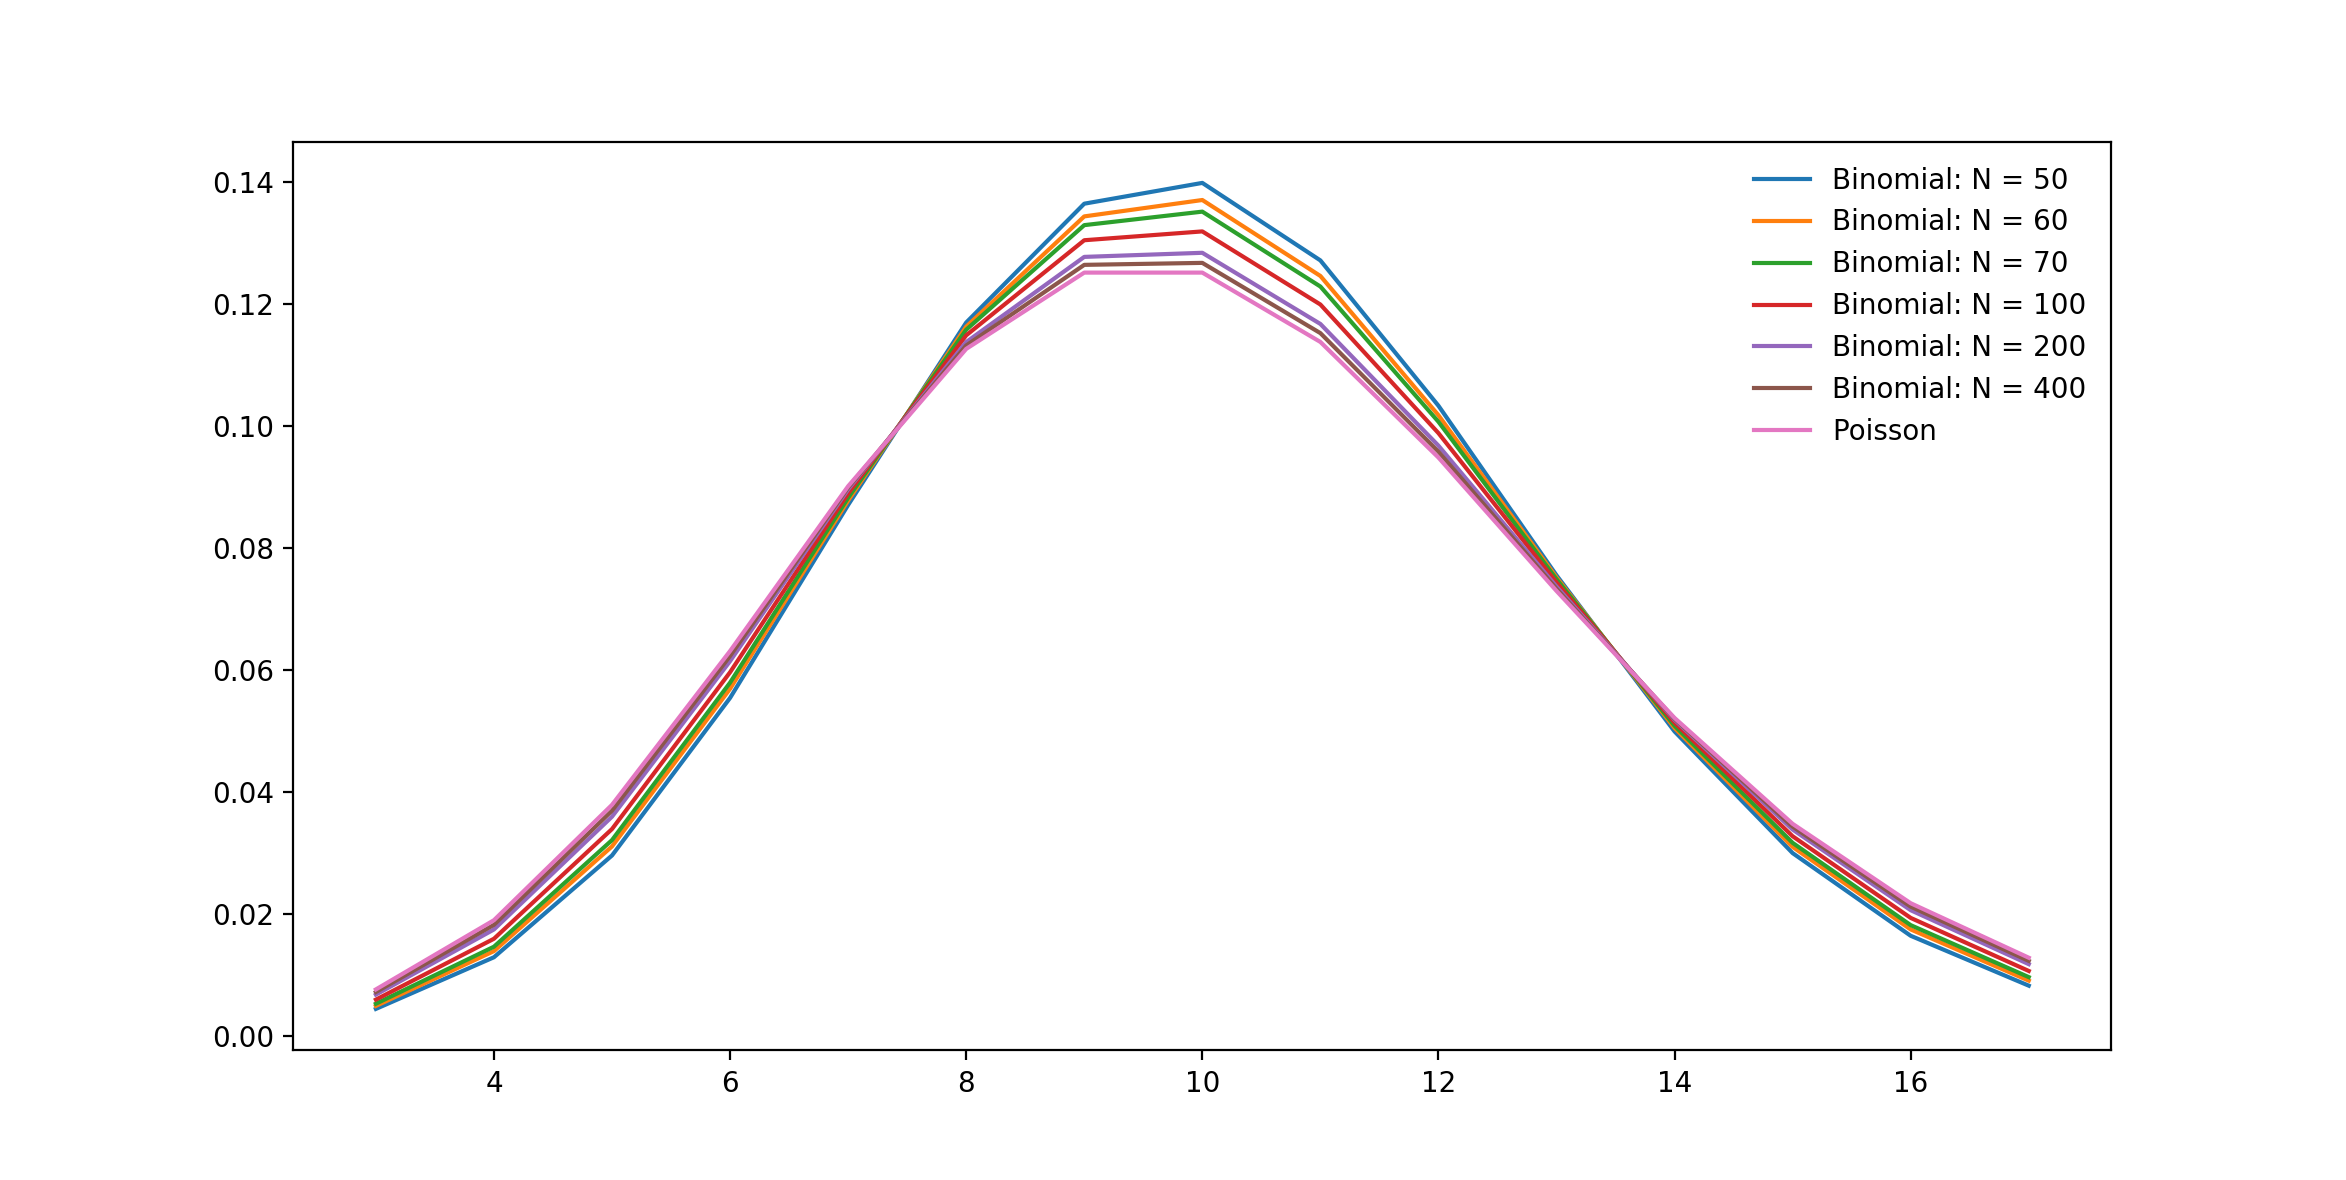
\includegraphics[width=\textwidth]{homework_02_fig.png}
            \caption{Binomial Distributions Approaching Poisson Distribution}
            \label{fig:binom_vs_poisson}
        \end{figure}

    \item[3.] And finally: a neat application to the Poisson distribution. A support center receives calls from customers who need help with some product. The calls arrive randomly and independently of each other, but historical data shows that the center receives on average $ 10 $ calls per hour. Beyond a certain number of calls in any given hour, the support line is overwhelmed and the system collapses, so the center needs to make sure to employ enough operators to handle occasional rushes.
        \subitem(a) At least how many calls does the support center have to be able to handle within an hour so that the probability of being overwhelmed is less than $ 0.1\% $?
        \begin{problem}
            To find this value, we need to find where the cumulative distribution function of the Poisson distribution is equal to $ 0.999 $. The cumulative distribution function for the Poisson distribution is
            \begin{equation}
                CDF = \frac{\Gamma(\lfloor n+1\rfloor, \mu)}{\lfloor n\rfloor!}
            \end{equation}
            where $ \Gamma(x,y) $ is the upper incomplete $\Gamma$ function and the $ \lfloor\rfloor $ symbols represent the floor function. From some guessing and checking, I've found this exceeds the tolerance at $ 21 $ calls per hour.
        \end{problem}
        \subitem(b) Repeat your calculation for three successively bigger call centers that receive on average $ 20 $, $ 50 $, and $ 100 $ calls per hour. Use your findings to argue why large call centers can be run more efficiently than small ones!
        \begin{problem}
            The $ 20 $ call-per-hour center needs to be able to handle $ 35 $ calls, the $ 50 $ call-per-hour center needs to be able to handle $ 73 $ calls, and the $ 100 $ call-per-hour center needs to be able to handle $ 132 $ calls. This number does not scale linearly with the average amount of calls received by the center, so larger call centers need to hire less people proportional to the amount of calls they get to handle rushes.
        \end{problem}
\end{itemize}

\end{document}
